\newpage
\usecaseristoratore{Termina prenotazione}
\label{usecase:Termina prenotazione}

\begin{figure}[h]
	\centering
	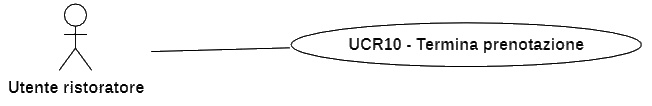
\includegraphics[width=0.9\textwidth]{./uml/UCR10.png} 
	\caption{Termina prenotazione}
	\label{fig:UCR10}
  \end{figure}

\begin{itemize}
	\item \textbf{Attore principale:} Utente ristoratore.

	\item \textbf{Precondizioni:}
	      \begin{itemize}
		      \item L'Utente ristoratore visualizza la prenotazione in dettaglio (vedi \autoref{usecase:Visualizza dettaglio lista prenotazioni}).
		      \item Tutti gli Utente base collegati alla prenotazione devono aver pagato il loro conto (vedi \autoref{usecase:Pagamento del conto}).
		      \item L'Utente ristoratore riceve la notifica dell'avvenuto pagamento (vedi \autoref{usecase:Visualizzazione notifica di avvenuto pagamento}).
	      \end{itemize}

	\item \textbf{Postcondizioni:} L'Utente ristoratore termina la prenotazione.


	\item \textbf{Scenario principale:}
	      \begin{enumerate}
		      \item L'Utente ristoratore seleziona l'opzione di terminazione della prenotazione;

		      \item Il Sistema aggiorna lo stato della prenotazione;
	      \end{enumerate}
\end{itemize}
